\documentclass[mathserif,hyperref={urlcolor=cyan,colorlinks=true}]{beamer}
\usepackage[utf8]{inputenc}

\usetheme{metropolis}

\usepackage{minted}
\usemintedstyle{tango}

\usepackage[T1]{fontenc}

\beamertemplatenavigationsymbolsempty
\setbeamertemplate{footline}{}

\definecolor{bgc}{HTML}{272822}

\newminted{perl}{fontsize=\fontsize{9}{9}}
\newminted{c}{fontsize=\fontsize{9}{9}}
\newminted{bash}{fontsize=\fontsize{9}{9}}

\title{Non-canonical XS Objects\\With a Bit of Perl Magic}
\author{Sergey Aleynikov}
\institute{Crazy Panda}
\date[May 2015]{YAPC::Russia 2015}
\begin{document}

\begin{frame}
\titlepage
\end{frame}

\begin{frame}[fragile]{Canonical XS objects}
\begin{ccode}
MODULE = DateTime   PACKAGE = DateTime

SV*
new(const char* CLASS)
CODE:
    DateTime* THIS = new DateTime();

    RETVAL = newRV_noinc(newSViv(PTR2IV(THIS)));
    sv_bless(RETVAL, gv_stashpv(CLASS, 0));
OUTPUT:
    RETVAL
\end{ccode}
\end{frame}

\begin{frame}[fragile]{Accessing canonical object}
\begin{ccode}
MODULE = DateTime   PACKAGE = DateTime

void
dump(SV* obj)
CODE:
    if (!sv_isobject(obj))
        croak("Not a DateTime object");

    DateTime* THIS = (DateTime*)SvIV(SvRV(obj));
    THIS->dump;
\end{ccode}
\end{frame}

\begin{frame}[fragile]{Write less with typemaps}
\begin{ccode}
typemap
DateTime* O_OBJECT

DateTime.xs
MODULE = DateTime   PACKAGE = DateTime

DateTime*
DateTime::new()
CODE:
    RETVAL = new DateTime();
OUTPUT:
    RETVAL

void
DateTime::dump()
CODE:
    THIS->dump();
\end{ccode}
\end{frame}

\begin{frame}{Why not?}
    \begin{columns}[c]
    \column{.5\textwidth}
        \begin{exampleblock}{Pros}
        \begin{itemize}
            \item Straightforward
            \item Inside a default typemap
            \item Fast unpack
        \end{itemize}
        \end{exampleblock}
    \column{.5\textwidth}
        \uncover<2->{
        \begin{alertblock}{Cons}
        \begin{itemize}
            \item No additional data
            \item One C object per Perl object
            \item Visible at Perl level
        \end{itemize}
        \end{alertblock}
        }
    \end{columns}
\end{frame}

\begin{frame}[fragile]{What is Perl magic?}
\begin{figure}
    \scalebox{0.35}{
        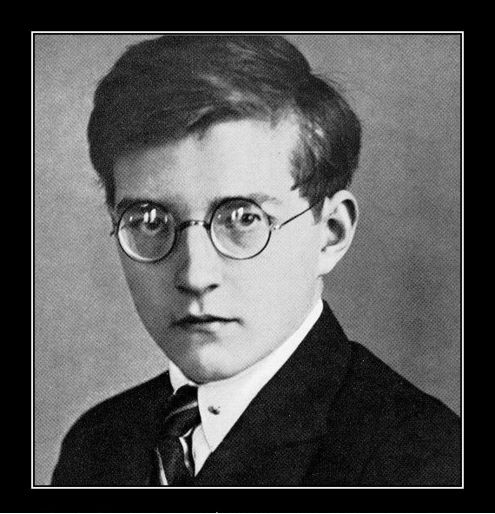
\includegraphics{Shostakovich.jpg}
    }
\begin{center}
{\bf
{\tiny
    \begin{verbatim}
    perl -e '$??s:;s:s;;$?::s;;=]=>%-{<-|}<&|`{;;y; -/:-@[-`{-};`-{/" -;;s;;$_;see'
    \end{verbatim}
}
}
\end{center}
\end{figure}
\end{frame}

\begin{frame}{What is Perl magic indeed?}
\begin{figure}
\scalebox{0.35}{
    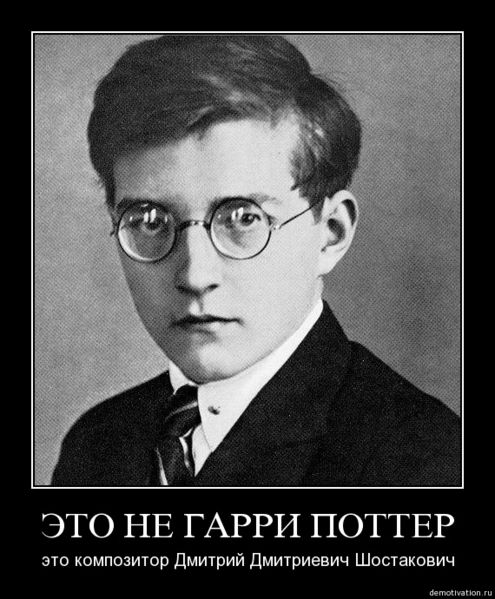
\includegraphics{Shostakovich_unv.jpg}
}
\end{figure}
\end{frame}

\begin{frame}{True magic}
\begin{itemize}
\item @ISA
\item \%\^{}H
\item \%SIG
\item \$!
\item \$DB::single
\item referee behind weaken()'d reference
\item tie()'d variable
\item ...more than 40 types
\end{itemize}
\end{frame}

\begin{frame}{How it works?}
\begin{itemize}
\item<1-> Acts on event trigger
    \begin{itemize}
    \item<1-> svt{\_}get
    \item<1-> svt{\_}set
    \item<1-> svt{\_}free
    \item<1-> svt{\_}clear
    \end{itemize}
\item<2-> Special types are checked at various places
\item<3-> PERL{\_}MAGIC{\_}ext reserved for extensions
\item<3-> sv{\_}magicext API call
\end{itemize}
\end{frame}

\begin{frame}[fragile]{Creating magical object}
\begin{ccode}
STATIC MGVTL marker;

MODULE = DateTime   PACKAGE = DateTIme

SV*
new(const char* CLASS)
CODE:
    SV* obj = newHV();
    DateTime THIS* = new DateTIme();
    sv_magicext(obj, NULL, PERL_MAGIC_ext, &marker,
        (const char*)THIS, 0);
    SvRMAGICAL_off(obj);

    RETVAL = newRV_noinc(obj);
    sv_bless(RETVAL, gv_stashpv(CLASS, 0));
OUTPUT:
    RETVAL
\end{ccode}
\end{frame}

\begin{frame}[fragile]{Accessing magical object}
\begin{ccode}
MODULE = DateTime   PACKAGE = DateTIme

void
dump(SV* obj)
CODE:
    if (!SvROK(obj)) croak("Not a DateTime object");

    MAGIC* mg = mg_findext(SvRV(obj), PERL_MAGIC_ext, &marker);
    if (!mg) croak("Not a DateTime object");

    DateTime THIS* = (DateTime*)(mg->mg_ptr);
    THIS->dump();
\end{ccode}
\end{frame}

\begin{frame}[fragile]{Lifecycle}
\begin{ccode}
MODULE = DateTime   PACKAGE = DateTIme

void
DESTROY(SV* obj)
CODE:
    MAGIC* mg = mg_findext(SvRV(obj), PERL_MAGIC_ext, &marker);
    if (mg) {
        DateTime THIS* = (DateTime*)(mg->mg_ptr);
        delete THIS;
    }
\end{ccode}
\end{frame}

\begin{frame}[fragile]{Example}
\begin{perlcode}
use DateTime;
use DDP;

my $foo = DateTime->new;
$foo->{bar} = 42;

$f->dump;
p $foo;
\end{perlcode}
\pause
\begin{bashcode}
% perl test.pl
dump
DateTime    {
    internals:  {
        bar 42
    }
}
\end{bashcode}
\end{frame}

\begin{frame}{Extending objects}
\begin{itemize}
\item Add data \& methods to pointer-based objects
\item Add data to perl hashes
\item Attach multiple C++ objects
\item Attach Perl data to CV*
\end{itemize}
\end{frame}

\begin{frame}{}
\begin{figure}
\scalebox{0.38}{
    
\includegraphics{jedi.jpg}
}
\end{figure}
\end{frame}

\begin{frame}[fragile]{Closures?}
\begin{perlcode}
__PACKAGE__->install_accessor("foo", $bar);
__PACKAGE__->install_accessor("bar", $baz);

sub install_accessor {
    my ($package, $name, $data) = @_;

    no strict 'refs';
    *{$package.'::'.$name} = sub {
        return $data;
    }
}
\end{perlcode}
\end{frame}

\begin{frame}[fragile]{Real magic}
%accessors as an example of additional data attached to XS
%point to XSANY.any_ptr unsafety
%CV* cv = newXS_flags(full_name_buf, CAIXS_inherited_accessor, __FILE__, NULL, 0);
%sv_magicext((SV*)cv, (SV*)keys_av, PERL_MAGIC_ext, &sv_payload_marker, NULL, 0);
%SvREFCNT_dec_NN((SV*)keys_av);
%note difference from previous magic installeri

\begin{ccode}
CV*
Perl_newXS_flags(pTHX_ const char* name, XSUBADDR_t subaddr,
    const char* const filename, const char* proto, I32 flags);

void
install_accessor(pTHX_ const char* name, SV* data) {
    CV* cv = newXS_flags(name, xs_accessor, __FILE__, NULL, 0);

#ifndef MULTIPLICITY
    CvXSSUBANY(cv).any_ptr = (void*)data;
#endif

    sv_magicext((SV*)cv, data, PERL_MAGIC_ext, &marker, NULL, 0);
    SvREFCNT_dec_NN(data);
    SvRMAGICAL_off((SV*)cv);
}
\end{ccode}
\end{frame}

\begin{frame}{}
\center{
    Questions?\\
    \vspace{2ex}
    github://\href{https://github.com/vovkasm/Class-Accessor-Inherited-XS}{Class::Accessor::Inherited::XS}\\
    \vspace{2ex}
    cpan://\href{http://search.cpan.org/~syber/Panda-XS/lib/Panda/XS.pm}{Panda::XS}
}
\end{frame}

\end{document}

